\documentclass[11pt]{article}
\usepackage[margin=1in]{geometry}
\usepackage{graphicx,booktabs,amsmath,xcolor,hyperref,caption,float}
\usepackage[T1]{fontenc}
\usepackage{lmodern}
\hypersetup{colorlinks=true,linkcolor=blue!50!black,citecolor=blue!50!black,urlcolor=blue!50!black}
\newcommand{\todo}[1]{\textcolor{red}{[TODO: #1]}}
\newcommand{\think}{\texttt{</think>}}
\newcommand{\Qwen}{Qwen3.5-0.8B}

\title{When AI Debugs AI: Repair or Bypass?\\An Audit of Weight Edits That End a Reasoning Loop}
\author{Chandrahas Aroori\\\small\texttt{chandrahas.aroori@gmail.com}}
\date{November 2026 \quad (draft v0.1)}

\begin{document}
\maketitle

\begin{abstract}
A frontier language model can end a small model's reasoning loop by editing its weights by hand, with no training. Takehi et al.\ call this weight-space programming and report one success, on math, in \Qwen{}.
We show that an edit can end the loop in two ways, and that accuracy does not tell them apart.
After a \emph{bypass} the model closes its thinking block at once, with no text in it, which the chat template already offers as a flag.
After a \emph{repair} the model still writes in its thinking block, and the block now closes.
Both words label behaviour that can be seen in answers; neither identifies a mechanism.
We give two tests. The first counts the characters before the \think{} tag in answers that an evaluation already has. The second gives every model the same answers that already loop and counts how many it closes.
We audit five edits of \Qwen{} on text-to-SQL, a task on which the model loops on 91\% of questions: the published math edit, two edits that Claude Fable 5.1 wrote in independent sessions of 25 forward passes each, and two gradient-descent baselines. The first test covers all five under greedy decoding. Sampled decoding, MATH-500 and the second test cover the math edit and the two Fable edits.
The math edit is a repair by both tests. Under the report's sampling settings, 139 of 150 SQL answers close thinking after a median of 16,145 characters, and the edit closes 57 of 60 looping answers that it is given, against 3 for the unedited model.
The edits made for SQL are bypasses. Under greedy decoding all 150 answers of each close at once. Each Fable edit closes 4 of the 60 looping answers, neither improves MATH-500 accuracy (9 of 100 correct against 8), and when the template supplies the closing tag neither scores above the unedited model (7.3\% and 8.0\% against 7.3\%).
Both sessions judged the editor by execution accuracy under greedy decoding. A bypass satisfies that criterion, and under greedy decoding the math edit closes thinking in only 22 of 150 answers. We ran no session that varies these properties, so we cannot separate them from the editor as the cause.
We do not contribute an editing method: the repair is the report's, and our editor's edits show no measured gain over a template flag. We contribute the tests, the audit, and two complete session traces.
We release the edits, all turn logs, the harness and the evaluation.
\end{abstract}

\section{Introduction}

Takehi et al.\ \cite{wsp} report that GPT-6 Astra, given a Python kernel over the weights of \Qwen{} and a budget of forward passes, raised the model's MATH-500 score from 7.9\% to 48.1\% by subtracting a ``loop direction'' from 130,188 entries in two MLP down-projection matrices.
They call the method weight-space programming, and we call their paper ``the report''.
No gradient was involved: the editor read activations, formed a hypothesis about why the model repeated itself, and wrote the fix by hand.
Public replications agree on where the gain comes from. The unedited model spends its token budget in a thinking loop, and the edited model finishes its answers \cite{hedwig,coletti,shapor,chalmers}.

A finished answer can come about in two ways, and this paper is about the difference.
After a \emph{bypass}, the model closes its thinking block at once, with nothing in it.
After a \emph{repair}, the model still writes in its thinking block, and the block now closes.
We use both words as labels for behaviour that can be seen in answers. Section~\ref{sec:setup} gives the exact test and its limit.
A bypass needs no weight edit, because the chat template of \Qwen{} can turn thinking off.
Both outcomes lower the loop rate and both can raise accuracy, so the numbers that evaluations of this method report do not separate them.

\begin{figure}[tbp]
\centering
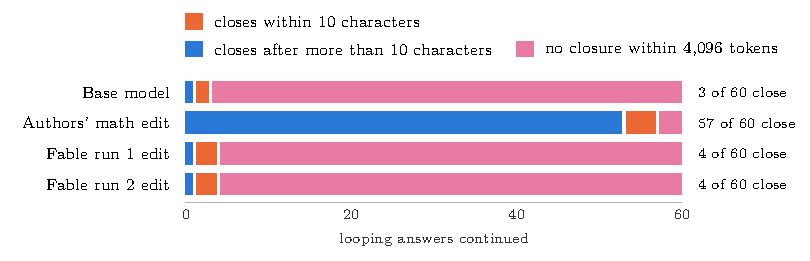
\includegraphics[width=0.9\textwidth]{fig/f5_continuation.pdf}
\caption{The continuation test. Each model receives the same 60 SQL answers of the unedited model, cut at the point where the answer already loops, and continues them for up to 4,096 tokens under the report's sampling settings. The report's math edit closes 57 of the 60 answers, 53 of them after more than 10 further characters. The two edits written by our editor close 4 each, against 3 for the unedited model.}
\label{fig:cont}
\end{figure}

We give two tests that separate the outcomes from generated text alone.
The first counts the characters between the start of the thinking block and the \think{} tag: zero means a bypass, and more than zero means the model wrote in the block and then closed it.
The second, the continuation test, starts each model after the first thinking position has passed. We take answers of the unedited model that already loop and let each edited model continue them (Figure~\ref{fig:cont}).
An edit that acts on a loop in progress should close these answers. An edit that only stops the model from entering the thinking block should not.

We then audit five edits of \Qwen{} on text-to-SQL, where the model with thinking enabled loops on 91\% of questions.
One is the report's released math edit, which was not written for SQL.
Two were written for SQL by Claude Fable 5.1 in independent sessions that follow the report's protocol.
Two are gradient-descent baselines restricted to the same weight entries as the Fable edits.
The math edit is a repair by the first test on SQL and on math, and by the continuation test on SQL.
The four edits made for SQL are bypasses by the first test. The continuation test, which we ran on the two Fable edits, agrees. When the template supplies the closing tag, the Fable edits show no accuracy gain over the unedited model.

Our own sessions therefore did not produce a repair, and we do not claim an editing method.
What the sessions do show is the conditions under which a bypass was returned twice. We judged the editor by execution accuracy under greedy decoding. A bypass satisfies that criterion, and under greedy decoding the math edit closes thinking in only 22 of 150 SQL answers. Both properties plausibly contributed. We ran no session that varies them, so we cannot separate them from the editor.
Our contributions:
\begin{enumerate}
\item Two tests that separate repair from bypass using only generated text: the character count before \think{}, and the continuation test (Section~\ref{sec:setup}).
\item An audit of five edits on SQL under greedy decoding, and of three of them under the report's sampling settings, on MATH-500 and in the continuation test, with a forced-tag control, random-location controls, and the same count applied to outputs that other groups released (Section~\ref{sec:sep}).
\item Two complete editor sessions on a new task, with every edit the editor tried and every prediction it stated, which show a frontier editor reaching a bypass after two failed attempts at a repair (Sections~\ref{sec:session} to~\ref{sec:what}).
\item A re-implementation of the harness that runs on one laptop, released with the edits and all turn logs.
\end{enumerate}

We use four more terms throughout. A \emph{lever} is any small weight change that alters a behaviour, whatever the explanation for it. An answer is \emph{cut} if it reaches the token limit. An answer \emph{loops} if some 40-character window of it, taken at steps of 20 characters, occurs five or more times. A \emph{footprint} is the set of weight entries that an edit changes.

\section{Setup}\label{sec:setup}

\begin{figure}[tbp]
\centering
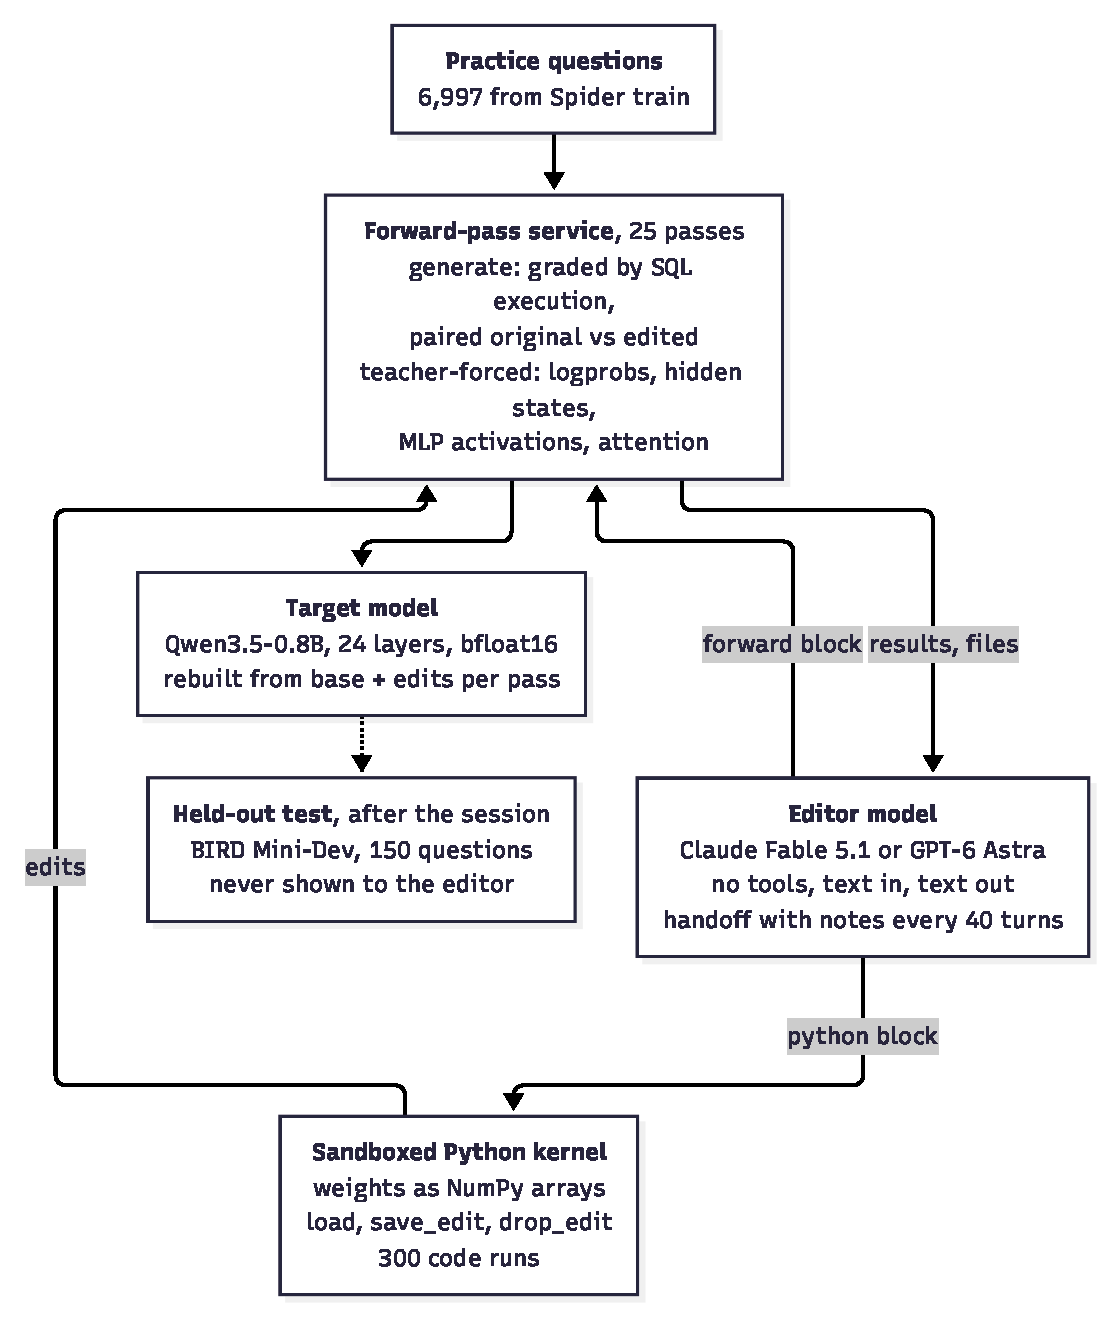
\includegraphics[width=0.95\textwidth]{fig/f1_setup.pdf}
\caption{The harness. The editor model has no tools of its own; it writes Python blocks that the harness runs in a sandboxed kernel over the weights, and forward requests that run the target model. The numbers of code runs and passes are budgets. Generation passes are graded by executing the produced SQL against the database; teacher-forced passes return log-probabilities, hidden states, MLP activations and attention. The held-out benchmark is never shown to the editor.}
\label{fig:setup}
\end{figure}

\paragraph{Target model.} \Qwen{} \cite{qwen35}: 24 layers, width 1,024, MLP width 3,584, vocabulary 248,320, tied embeddings. Six layers (3, 7, 11, 15, 19, 23) use full attention; the others use gated linear attention. Weights are bfloat16 safetensors; the editor reads and writes them as float32 NumPy arrays and the harness casts edits back to bfloat16.

\paragraph{Task and obstacle.} Text-to-SQL: the user message gives a SQLite schema and a question; the answer is graded by executing the produced query and comparing result sets with the gold query. With thinking enabled through the chat template, \Qwen{} writes ``Thinking Process: 1.\ Analyze the Request \ldots\ 2.\ Analyze the Schema \ldots'' and then repeats schema bullets until the 8,192-token limit. On 150 BIRD Mini-Dev questions \cite{bird} (every third question, indices 0 to 447, covering 10 of the 11 databases), greedy decoding: 0.7\% correct, 98.7\% cut at the limit, 90.7\% with a visible repetition (a 40-character window that occurs five or more times). This is the same failure class the report fixes on math, in a domain where, under greedy decoding, the report's edit mostly does not transfer (Table~\ref{tab:main}; Section~\ref{sec:sep} shows that this depends on the decoding).

\paragraph{Practice and test.} The editor sees practice questions only: 6,997 from Spider train \cite{spider}, with gold SQL and databases. The held-out test is BIRD Mini-Dev (500 questions over 11 databases); thinking-mode evaluations use 150 evenly spaced questions because each looping answer costs 8,192 tokens.

\paragraph{Budgets and rules.} These follow the report: 25 forward passes, 300 code runs, a handoff every 40 turns in which the conversation restarts with the task, the editor's notes file and its current edit list, and a final answer when the passes are spent. A generation pass answers up to 128 practice questions (64 per model in a paired ``both'' request) with greedy decoding and 8,192 new tokens; a teacher-forced pass, in which the model reads a given text and returns its internal values without generating, covers up to 1,024 texts. Gradient descent, running the model inside the kernel, and edits to the final norm, the embeddings, or whole-tensor rescaling are refused. The kernel is sandboxed (no network; writes only inside the run directory).

\paragraph{Editor.} Claude Fable 5.1, called headless with tools, user settings and memory disabled, reasoning effort at its highest setting, one conversation per handoff. The report used GPT-6 Astra; we keep that path for the editor-dependence runs. \todo{Astra runs}

\paragraph{Evaluation after the session.} The submitted edit replaces the original tensors; the model is run with mlx-lm, greedy, 8,192 new tokens, thinking enabled, on the same 150 BIRD questions as the baseline. We report execution accuracy, the share of answers cut at the token limit, the loop share, and paired wrong-to-right and right-to-wrong counts against the base model on the same questions.

\paragraph{The edits under audit.} Five edits, all of MLP down-projection columns. The \emph{math edit} is the report's released edit: 130,188 entries in layers 15 and 19, written for MATH-500. The \emph{Fable run 1 edit}, which Sections~\ref{sec:session} and~\ref{sec:results} call edit C, changes 4,083 entries on four neurons in layers 17 to 20. The \emph{Fable run 2 edit} changes 2,048 entries on two neurons in layers 16 and 18. The two \emph{gradient baselines} train only the entries of one Fable edit each, toward the target \think{} followed by the gold SQL. Section~\ref{sec:session} describes how the editor arrived at its edits; the audit in Section~\ref{sec:sep} needs only the edited weights. Test 1 under greedy decoding covers all five edits. Sampled decoding, MATH-500, the continuation test and the forced-tag control cover the math edit and the two Fable edits; the gradient baselines were run on SQL under greedy decoding only.

\paragraph{Test 1: characters before the closing tag.} For each answer we record whether it contains \think{}, and the number of characters between the start of the thinking block and the tag, after leading and trailing white space is removed. An answer \emph{closes at once} if that number is zero. The \emph{first thinking position} is the position of the first token that the model generates after the template's opening \texttt{<think>} tag and newline. We call an edit a bypass if its answers close at once and a repair if they close after text. What sustains a loop cannot be read from outputs, so this is a test of behaviour. Text in the block is not proof of reasoning, since it can be filler or the end of a repeated fragment, and an empty block does not prove that no computation took place. The test does not show which mechanism an edit changed, and every use of ``repair'' in this paper carries that limit.

\paragraph{Test 2: continuation.} We take the unedited model's sampled answers to the 150 held-out questions and keep those that were cut, never closed thinking, and loop. For each we find the first length, in steps of 1,000 characters, at which the text already loops, and keep the text up to that length as a prefix. Of the 96 answers that qualify we use the first 60. Their prefixes are 9,000 to 32,000 characters long, with a median of 17,500, and come from 6 databases. Every model then receives the same prompt followed by the same prefix, and generates up to 4,096 more tokens under the report's sampling settings. We count the continuations that reach \think{}. The prefix is text and not internal state: each model reads the prefix with its own weights, so the test measures what an edited model does when it is given a looping answer.

\paragraph{Decoding.} Greedy decoding makes paired comparisons exact, and both editor sessions and their controls used it. The report samples: temperature 0.6, top-$p$ 0.95, top-$k$ 20, presence penalty 1.5. We call these the report's sampling settings and run the audit under both. Runs with thinking off use the model card's settings (temperature 0.7, top-$p$ 0.8).

\section{The audit}\label{sec:sep}

\begin{table}[tbp]
\centering
\begin{tabular}{lrrr}
\toprule
Condition (thinking on, $n{=}150$) & Closes & At once & Median chars before \think{} \\
\midrule
Base & 2 & 0 & 3,092.5 \\
Authors' math edit \cite{wsp} & 22 & 0 & 5,768 \\
Fable run 1 edit & 150 & 150 & 0 \\
Fable run 2 edit & 150 & 150 & 0 \\
Gradient descent, run 1 footprint & 150 & 150 & 0 \\
Gradient descent, run 2 footprint & 150 & 150 & 0 \\
\bottomrule
\end{tabular}
\caption{Test 1 under greedy decoding. ``Closes thinking'' counts answers that contain \think{}; the median is over those answers.}
\label{tab:sep}
\end{table}

\begin{figure}[tbp]
\centering
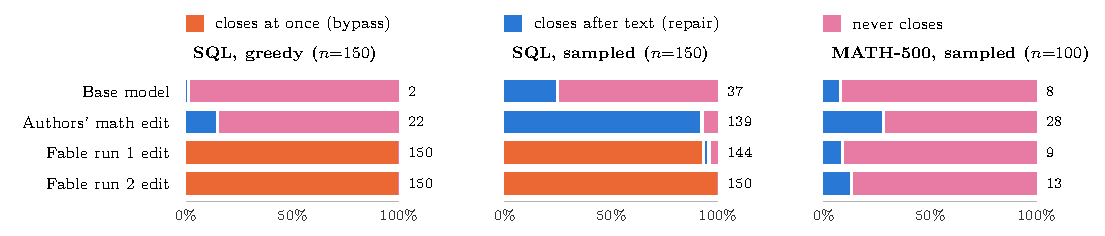
\includegraphics[width=\textwidth]{fig/f4_outcomes.pdf}
\caption{How the thinking block ends, as a share of answers, for the base model and three edits. The number at the right of each bar is the count of answers that close thinking. Under greedy decoding the math edit looks ineffective on SQL; under the report's sampling it ends the loop after reasoning. The Fable edits close thinking at once on SQL and have no visible effect on MATH-500. Data: Tables~\ref{tab:sep} and~\ref{tab:samp}.}
\label{fig:outcomes}
\end{figure}

\paragraph{Test 1 under greedy decoding.} The four edits made for SQL close thinking in all 150 answers, and all 150 close at once (Table~\ref{tab:sep}, Figure~\ref{fig:outcomes}). These edits leave the thinking block empty. The math edit does the opposite on a small share of answers: 22 of 150 close thinking, and all 22 do so after text, with a median of 5,768 characters. Under greedy decoding the math edit therefore looks like a weak repair that mostly fails to transfer to SQL.

\paragraph{Test 1 under the report's sampling settings.} Greedy decoding hid most of the math edit's effect (Table~\ref{tab:samp}). With the settings the edit was built under, cut answers fall from 75.3\% to 8.0\%, and 139 of 150 answers close thinking, none at once, after a median of 16,145 characters. The text before \think{} is mostly not a loop that happened to end: 9 of the 139 blocks loop by our definition, and all 16 correct answers come from answers that closed thinking. The Fable edits stay bypasses under sampling: 140 of 150 and 150 of 150 answers close at once.

On MATH-500 the roles do not reverse. The math edit closes thinking in 28 of 100 answers against 8 for the unedited model, none at once. The Fable edits are not bypasses there and show no accuracy gain: no answer closes at once, 9 of 100 answers are correct for each against 8, and 91 and 89 are cut against 92. Their loop shares are higher than the unedited model's (79\% and 88\% against 73\%), a difference we have not examined. The repair, written for math, carries over to SQL. The bypass, written for SQL, does not carry over to math.

\begin{table}[h]\centering\small
\begin{tabular}{llrrrr}
\toprule
Task & Condition & Correct \% & Cut \% & Close thinking & At once \\
\midrule
BIRD, $n{=}150$ & Base, thinking on & 5.3 & 75.3 & 37 & 0 \\
 & Base, thinking off & 6.7 & 0.7 & -- & -- \\
 & Authors' math edit & 10.7 & 8.0 & 139 & 0 \\
 & Fable run 1 edit & 2.0 & 4.7 & 144 & 140 \\
 & Fable run 2 edit & 2.7 & 0.7 & 150 & 150 \\
\midrule
MATH-500, $n{=}100$ & Base, thinking on & 8 & 92 & 8 & 0 \\
 & Base, thinking off & 42 & 33 & -- & -- \\
 & Authors' math edit & 21 & 72 & 28 & 0 \\
 & Fable run 1 edit & 9 & 91 & 9 & 0 \\
 & Fable run 2 edit & 9 & 89 & 13 & 0 \\
\bottomrule
\end{tabular}
\caption{The report's sampling protocol. BIRD at 8,192 tokens; MATH-500 at 16,384 tokens with thinking on and 8,192 with thinking off. Thinking-off rows use model-card sampling on both tasks. One seed.}
\label{tab:samp}
\end{table}

\paragraph{Test 2: the math edit closes looping answers that it is given.} Test 1 leaves one doubt. An edit could prevent loops from starting without acting on a loop once it runs. The continuation test addresses that doubt (Figure~\ref{fig:cont}). The math edit closes 57 of the 60 looping answers, and the median text it writes first is 2,625 characters. How many of these count as further writing depends on the threshold: 53 continuations write more than 10 characters before the tag, 47 more than 50, 45 more than 100, and 35 more than 1,000. The shortest only finish a sentence, for example ``6 sentences long.'' The unedited model closes 3 of the same 60 answers and the Fable edits close 4 each, a difference of one answer that we do not interpret. Cut continuations fall from 56 of 60 to 4 for the math edit and stay at 55 and 56 for the Fable edits. The Fable result is what their design predicts: in both edits the neurons that write the closing-tag direction fire only at the first thinking position, and in this test that position has passed.

The continuations of the math edit are also more often right. 8 of its 60 answers are correct against 2 for the unedited model, and on paired questions the math edit is right where the unedited model is wrong on 6 and the reverse on none (exact McNemar $p = 0.031$). All 8 come from continuations that closed thinking.

\paragraph{With the tag supplied, the Fable edits show no accuracy gain.} If a Fable edit only writes the closing tag, then supplying the tag through the template should make the edit redundant. We ran both Fable edits with thinking turned off in the template, which inserts an empty \texttt{<think></think>} block (Table~\ref{tab:flag}). Accuracy, cut share and loop share are within two questions of the unedited model in the same mode. This is a failure to find a difference at $n = 150$ and not a test of equivalence. Under greedy decoding the run 1 edit produces the same text as the unedited model, character for character, on 106 of 150 questions. The run 2 edit does so on 6, because one of its two neurons fires on every token; it changes whether the answer is correct on 13 questions, and its accuracy is within one question of the unedited model's. With thinking on, the edits are not identical to the flag: under greedy decoding the run 1 edit leaves 41 of 150 answers cut against 18 for the flag (Section~\ref{sec:results}).

\begin{table}[h]\centering\small
\begin{tabular}{lrrrrr}
\toprule
 & \multicolumn{3}{c}{Greedy} & \multicolumn{2}{c}{Sampled} \\
Thinking off, $n{=}150$ & Correct \% & Cut \% & Loop \% & Correct \% & Cut \% \\
\midrule
Unedited & 7.3 & 12.0 & 10.7 & 6.7 & 0.7 \\
Fable run 1 edit & 7.3 & 12.7 & 10.7 & 6.0 & 0.0 \\
Fable run 2 edit & 8.0 & 11.3 & 10.7 & 5.3 & 0.0 \\
\bottomrule
\end{tabular}
\caption{The forced-tag control. Thinking is turned off in the chat template, so the template writes the closing tag. BIRD, 8,192 tokens; the sampled columns use the model card's settings.}
\label{tab:flag}
\end{table}

\paragraph{Moving the math edit to random neurons lowered closure in three draws, and accuracy does not show it.} We moved the math edit's change vectors to randomly chosen neurons in the same layers, three draws, and ran each on 50 questions under the report's sampling settings. The draws close thinking in 6, 22 and 19 of 50 answers (12\% to 44\%). The real edit closes 139 of 150 (93\%) and the unedited model 37 of 150 (25\%). The 50 control questions are every tenth question of the benchmark and share only 15 questions with the 150, so the comparison is between rates on overlapping samples and not a paired one. On the 15 shared questions the counts are 14 for the edit, 6 for the unedited model, and 1, 7 and 8 for the draws. Accuracy does not separate these conditions: the draws score 8\%, 18\% and 10\% against 10.7\% for the edit. At this sample size, and with three draws and one seed, the closing count separates the edit from the draws and accuracy does not.

\paragraph{Accuracy.} On the 150 questions under sampling, 16, 10 and 8 answers are correct for the math edit, thinking off and the unedited model, and 3 and 4 for the two Fable edits. On paired questions the math edit is right where the unedited model is wrong on 13 and the reverse on 5 (exact McNemar $p = 0.096$), and against thinking off the counts are 11 and 5 ($p = 0.21$). Neither difference is significant. The math edit does beat both bypass edits: 14 against 1 for run 1 ($p = 0.001$) and 14 against 2 for run 2 ($p = 0.004$). These four $p$-values are not corrected for multiple comparisons. The math edit's 21\% on MATH-500 is below the published 48\%. Our limit is 16,384 tokens, half the report's, and 72 of 100 answers reach it. The limit is a plausible contributor, and the two set-ups differ in other ways that we have not matched.

\paragraph{Test 1 on other groups' outputs.} Test 1 needs only generated text, so it applies to answers that others have released. On the math outputs of an independent replication \cite{chalmers} (50 problems, three seeds, the report's sampling settings, 16,384 tokens), 16 of 150 base answers close thinking, and 125 of 150 answers of the report's edit do; none closes at once, and the median text before \think{} is 23,790 characters for the edit. That replication's random-direction control on the same 64 neurons per layer closes thinking in 30 of 150 answers, none at once. The authors' own released sample \cite{wsp} (20 MATH-500 problems, 32,768 tokens) gives 1 of 20 for the base model and 18 of 20 for the edit, none at once. By the operational test the math edit is a repair on its own task in other groups' data, as it is on SQL in ours, and no released condition on math is a bypass.

A second signature of the difference is known from those releases. A bypass should match the template flag it imitates, while a repair can exceed it. Independent evaluations of the math edit report 50.2\% on MATH-500 with thinking on against 45.8\% for the unedited model with thinking off \cite{coletti}. Those analyses ask whether the edit adds ability; none asks which of the two outcomes it is.

\section{How the editor reached a bypass}\label{sec:session}

The audit above needs only the edited weights. This section and the next record where the two Fable edits came from, because the path shows the conditions under which a bypass was returned.

\begin{figure}[tbp]
\centering
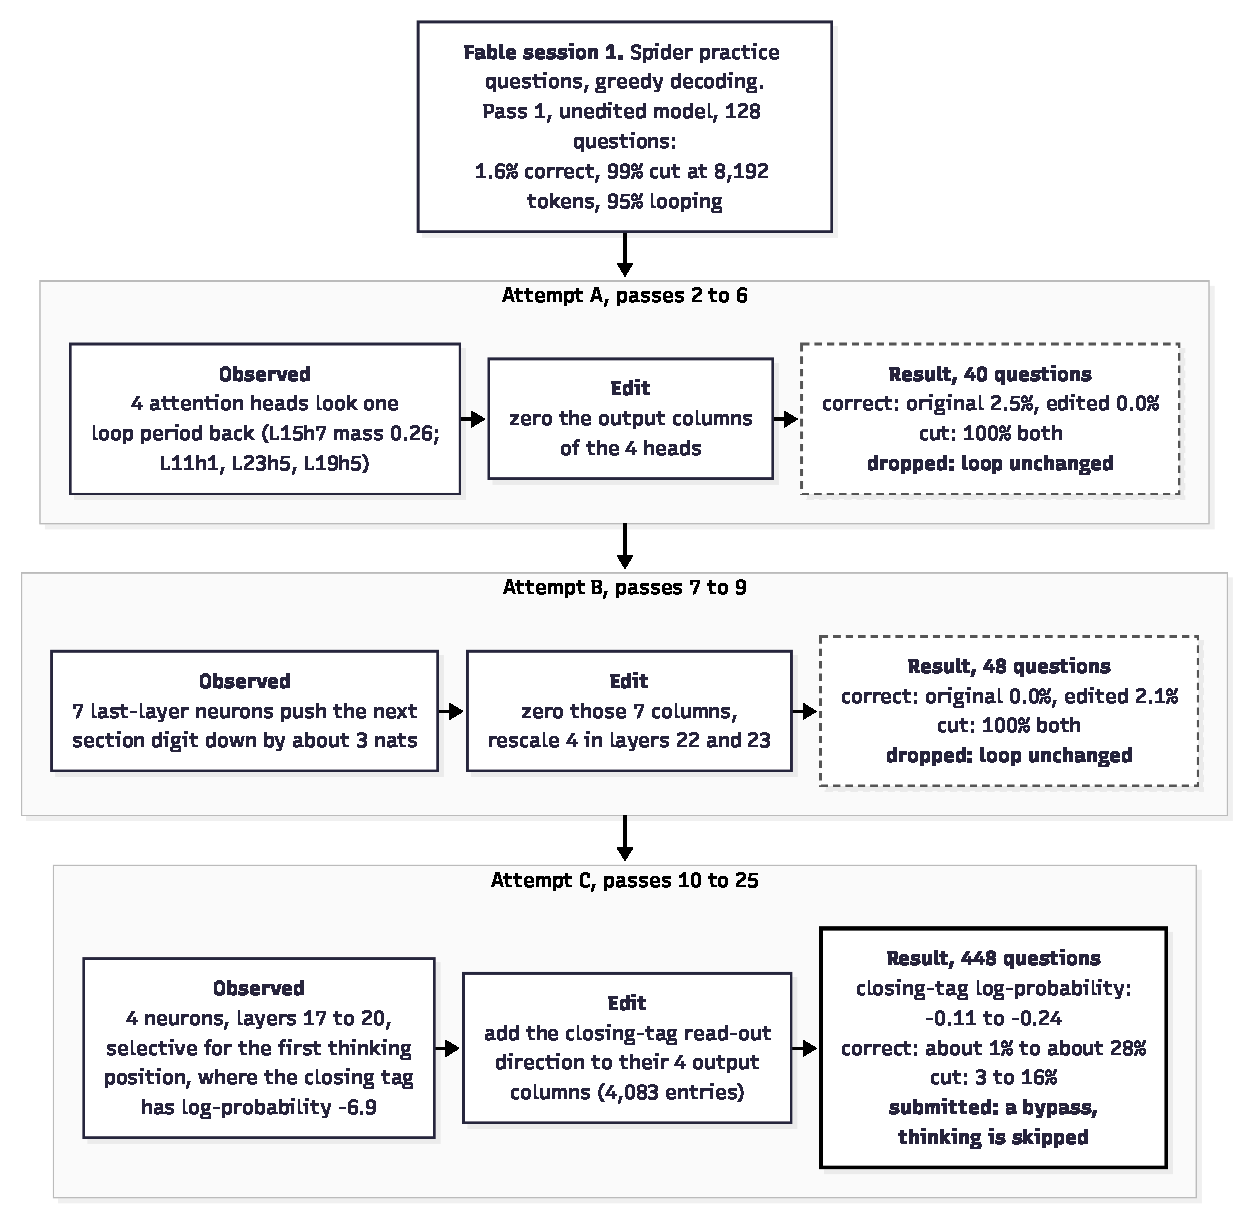
\includegraphics[width=0.95\textwidth]{fig/f2_session.pdf}
\caption{Fable session 1: three observations, three edits, one submitted. Each row reads left to right. Dashed boxes are edits the editor dropped; the bold box is the submitted edit, which is a bypass and not a repair of the loop. Pass numbers refer to the forward-pass budget; code runs and handoffs are omitted. All numbers are the editor's own measurements on practice questions under greedy decoding.}
\label{fig:session}
\end{figure}

The session ran 9.8 hours on one laptop (328 turns, 299 code runs, 25 passes, 9 handoffs; 493k output tokens from the editor). Figure~\ref{fig:session} summarises it; the editor's notes file and all turns are released.

\paragraph{Attempt 1: induction heads.} After one diagnostic generation pass (1.6\% correct, 99\% cut, 95\% looping), the editor teacher-forced two loop transcripts with attention saved at the six full-attention layers. In the loop region it found heads that put attention mass one period back, the signature of induction heads \cite{induction}: layer 15 head 7 at 0.26 mass, then layer 11 head 1, layer 23 head 5 and layer 19 head 5. It also measured that the loop is ``soft'': at each bullet start the copied token leads the best alternative by a median 1.6 nats, and greedy decoding always takes the copy. Its edit zeroed the output-projection columns of the four heads. Paired generation on 40 fresh problems: original 2.5\%, edited 0.0\%, both 100\% cut. The editor dropped the edit. Layer 15 head 7 is, as it happens, the head the report's p25c run zeroed for math; here it did nothing.

\paragraph{Attempt 2: digit-suppressing neurons.} The editor then teacher-forced six of the model's own loop transcripts with hidden states and MLP activations in layers 16 to 23, and asked a sharper question: at each blank line the model chooses between ``indent and add another bullet'' and ``write the next section number''. It found seven neurons in the last layer's MLP that fire when a digit is about to be predicted and push that exact digit down by about 3 nats (n580 for `3', n598 for `5', n564 for `4', n557 for `1', n485 for `2', n669 for `6', n639 for `7'), plus three neurons that move the newline decision. Its edit zeroed the seven columns and rescaled four others in layers 22 and 23. Paired generation on 48 fresh problems: original 0.0\%, edited 2.1\%, both 100\% cut. Dropped. The editor's note at this point reads: ``The looping is distributed and not fixable at one site.''

\paragraph{Attempt 3: the start-of-thinking switch.} The editor changed the question from ``why does the loop continue'' to ``why does the model enter this mode at all''. At the first thinking position, right after the \texttt{<think>} tag and newline, \think{} is already a plausible continuation (log-probability $-6.9$, rank 6 to 8), and direct logit attribution shows the MLPs of layers 16 to 23 pushing against it diffusely, by about 9 nats in total. It then searched for neurons selective to that position and found four, one each in layers 17 to 20 (n537, n628, n2424, n1235), with activations 1.2 to 2.7 there and a 99.9th-percentile magnitude elsewhere of 0.3 to 0.7. The edit adds to each neuron's down-projection column a multiple $\alpha$ of the unit vector $u = \mathrm{unit}(\gamma \odot E[\think])$, where $\gamma$ is the final norm gain and $E$ the tied unembedding, with $\alpha = 0.20, 0.20, 0.25, 0.15$ (Figure~\ref{fig:mechanism}). 4,083 entries change; the largest change is 0.039.

\begin{figure}[tbp]
\centering
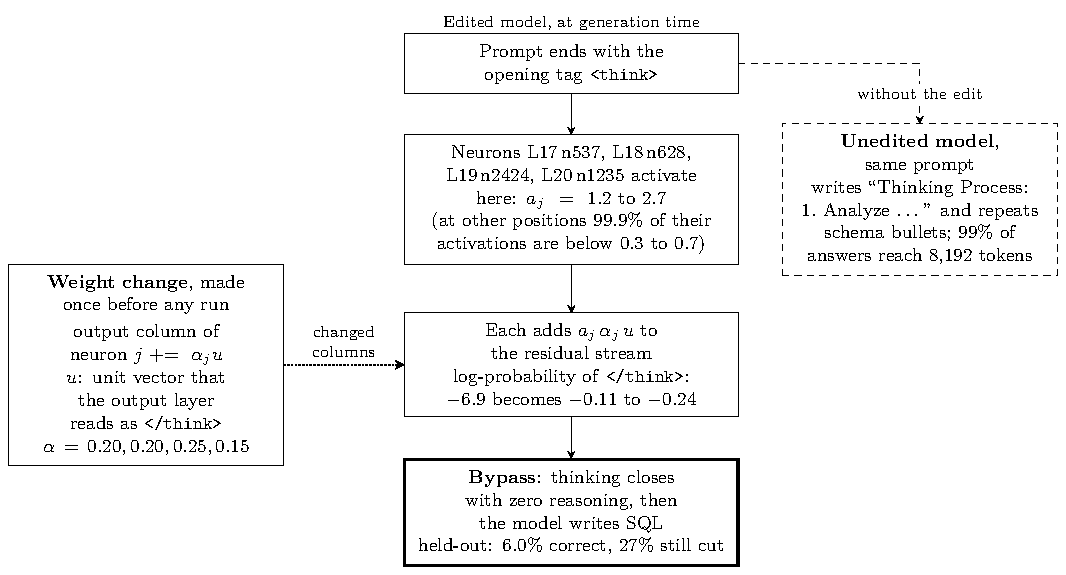
\includegraphics[width=0.95\textwidth]{fig/f3_mechanism.pdf}
\caption{The submitted edit. The weights are changed once (left). At generation time, four MLP neurons that are selective for the first thinking position then write the \think{} read-out direction into the residual stream, and the model closes its thinking with no reasoning (centre). The unedited model on the same prompt loops (right, dashed).}
\label{fig:mechanism}
\end{figure}

Teacher-forced, the log-probability of \think{} at the first position rose from $-6.9$ to between $-0.11$ and $-0.24$, including on a 4,196-token prompt and on BIRD-style prompts with a hint line. The editor then spent its remaining passes on confirmation: seven paired sets of 64 fresh practice problems, 448 in total, original about 1\% and edited about 28\%, a gain of 26.8 points with every set between 18.8 and 31.3 points and 3 to 5 standard errors above zero; 122 problems went wrong to right and 2 right to wrong; cut answers fell from about 100\% to 3 to 16\%. A variant that wrote the direction of the token `Okay' instead, to start free-form thinking rather than close it, scored 3.1\% with 98\% cut, and was dropped.

\section{Held-out results and controls}\label{sec:results}

\begin{table}[tbp]
\centering
\resizebox{\textwidth}{!}{%
\begin{tabular}{llrrrrr}
\toprule
Condition & Entries & $n$ & Acc.\ \% & Cut \% & Loop \% & W$\to$R / R$\to$W \\
\midrule
Base, thinking on & 0 & 150 & 0.7 & 98.7 & 90.7 & \\
Base, thinking off via template, 8,192 tokens & 0 & 150 & 7.3 & 12.0 & 10.7 & \\
Base, thinking off, 1,024 tokens, all questions & 0 & 500 & 7.0 & 14.0 & 9.0 & \\
Authors' math edit \cite{wsp}, thinking on & 130,188 & 150 & 3.3 & 87.3 & 82.0 & 5 / 1 \\
\midrule
Fable edit C (this work), thinking on & 4,083 & 150 & \textbf{6.0} & 27.3 & 26.0 & 9 / 1 \\
Random location, same footprint, 5 draws & 4,083 & 5$\times$50 & 0.0 to 2.0 & 100 & 90 to 98 & \\
Gradient descent on the same 4,083 entries & 4,083 & 150 & 4.7 & 30.7 & 29.3 & 7 / 1 \\
\midrule
Fable run 2 edit, thinking on & 2,048 & 150 & 5.3 & 25.3 & 24.0 & 8 / 1 \\
Random location, run 2 footprint, 5 draws & 2,048 & 5$\times$50 & 0.0 to 4.0 & 94 to 100 & 86 to 96 & \\
Gradient descent on the run 2 footprint & 2,048 & 150 & 7.3 & 29.3 & 29.3 & 11 / 1 \\
\midrule
Fable edit A (induction heads), practice & \todo{} & 40 & 0.0 & 100 & 100 & \\
Fable edit B (digit neurons), practice & \todo{} & 48 & 2.1 & 100 & 100 & \\
\bottomrule
\end{tabular}}
\caption{BIRD Mini-Dev, greedy, 8,192 new tokens unless stated, the same 150 evenly spaced questions in every 150-question row. ``Cut'' is the share of answers that hit the token limit; ``Loop'' the share with a visible repetition. The last column is the paired count of questions that changed outcome against the base model on the same questions. Edits A and B were only evaluated on practice questions inside the session. \todo{two Astra runs as further rows}}
\label{tab:main}
\end{table}

\paragraph{The edit transfers.} On BIRD, which the editor never saw and whose prompts are longer and carry a hint line, edit C removes the thinking loop: cut answers fall from 98.7\% to 27.3\% and loops from 90.7\% to 26.0\%. Accuracy rises from 0.7\% to 6.0\%, with 9 questions wrong to right and 1 right to wrong. Of the 41 answers that are still cut, 39 loop, now inside the SQL itself (errors such as ``too many FROM clause terms''), which the base model also produces with thinking off.

\paragraph{The neuron choice mattered.} Five edits that apply the same four change vectors to randomly chosen neurons in the same four layers leave the model where it was: 0 to 2\% correct, 100\% cut, 90 to 98\% looping. The editor picked four neurons out of 14,336 candidates in those layers and the pick was not interchangeable.

\paragraph{The edit is worth about one template flag.} The base model with thinking disabled through the chat template, same 150 questions and token limit, scores 7.3\% with 12.0\% cut and 10.7\% looping. Accuracy is indistinguishable from the edit (6.0\%, 95\% Wilson interval 3.2 to 11.0, against 7.3\%, interval 4.1 to 12.7), but the edit leaves about twice as many cut answers (27.3\%, interval 20.8 to 35.0, against 12.0\%, interval 7.7 to 18.2); we have not explained that gap. The chat template with thinking off inserts an empty \texttt{<think></think>} block, and the edit makes the model emit the closing tag itself, so the two conditions differ in whether the tag comes from the template or from the weights. The edited weights also stay in place while the SQL is written, which may account for the extra cut answers.

\paragraph{Gradient descent can realise the same bypass on the same entries.} We trained only the same 4,083 entries with Adam (250 steps, batch 2, learning rate $2\times10^{-4}$, rows capped at 1,024 tokens) on practice questions, with the target \think{} followed by the gold SQL. The result behaves like edit C: every one of the 150 BIRD answers opens with \think{}, accuracy is 4.7\%, cut 30.7\%, loop 29.3\%, paired 7 wrong to right and 1 right to wrong. The change vectors are about twice as long as the editor's (norms 0.38 to 0.41 against 0.15 to 0.25) and nearly orthogonal to its direction $u$ (cosine 0.01 to 0.12). The training target prescribes the bypass, so this baseline shows that the footprint is sufficient for an optimiser to realise it, not that an optimiser would choose a bypass unprompted. Given the footprint and the target, an optimiser reaches the same behaviour by a different route; what the editor contributed that the optimiser did not is the choice of the four neurons.

\paragraph{A second session converges on the bypass, not on the neurons.} A second Fable session, with a fresh conversation and no shared notes, also concluded that the loop could not be removed at one site and also went for the entry into thinking. It replaced the output column of one neuron, layer 18 neuron 2800, which fires only at the first thinking position, with a direction that drives \think{}, and wrote a constant steering direction (the residual-stream difference induced by an in-context instruction to keep the query simple) into layer 16 neuron 3, which fires on every token. On 192 fresh practice problems: 1.6\% to 28.1\%, 51 wrong to right, 0 right to wrong. On BIRD: 5.3\% correct, 25.3\% cut, 24.0\% looping. None of its neurons is one of the first session's four. Random-location draws do nothing, and gradient descent on its 2,048 entries again realises the bypass (7.3\%, every answer opening with \think{}).

\section{What the trace says about the method}\label{sec:what}

\paragraph{Understanding versus finding a lever.} Two readings of a successful session are possible. In the first, the editor understood a mechanism and repaired it. In the second, the editor searched until some small weight change stopped the loop, and the mechanistic account came along with it. Session 1 contains three mechanistic hypotheses about the loop. The editor backed each with a measurement, turned each into a precise edit, and tested each on generation with fresh practice questions. It did not write down a forecast for the first two edits, so we read each edit as the claim that changing these components would stop the loop. Both claims failed: the loop rate did not move. That does not show the components are uninvolved, because redundancy or compensation can hide a real role. The third hypothesis was correct, but it is a claim about entry into the thinking mode and not about what sustains the loop. The first reading predicted that edits A and B would reduce looping, and they did not. The second predicted that some small weight set would work whatever the explanation; edit C did, and so did gradient descent on its footprint. The editor described its own result accurately in its final answer: ``skip the degenerate Thinking Process loop and answer directly''.

\paragraph{Calibration.} We extracted every statement in the turn logs of both sessions in which the editor predicted a result before seeing it (\texttt{analysis/calibration\_r1.json}, \texttt{calibration\_r2.json}; each quote is verified verbatim against its turn). There are few: 20 per session in about 330 turns, because the editor writes mostly code and its hidden reasoning is not logged, so the counts are a lower bound (Table~\ref{tab:calib}). Three things stand out. Predictions about the local effect of an edit on log-probabilities were reliable: 8 of 10 confirmed and none refuted. Predictions about what a diagnostic measurement would show differ sharply between sessions, 1 of 10 confirmed in the first and 13 of 15 in the second. And neither session stated in advance what edits A or B would do to generated answers; the only generation predictions are that the bypass edit makes answers skip thinking (confirmed) and that the practice gain will transfer to the benchmarks (not testable inside the session; on BIRD the 28\% became 6\%). The editor committed to forecasts where it was on firm ground and did not commit where the method's central claim is tested.

\begin{table}[h]\centering\small
\begin{tabular}{llrrrr}
\toprule
Session & Prediction about & Confirmed & Partly & Refuted & Untested \\
\midrule
1 & edit, log-probabilities & 6 & 1 & 0 & 0 \\
 & edit, generated answers & 2 & 0 & 0 & 1 \\
 & diagnostic measurement & 1 & 4 & 5 & 0 \\
\midrule
2 & edit, log-probabilities & 2 & 1 & 0 & 0 \\
 & edit, generated answers & 1 & 0 & 0 & 1 \\
 & diagnostic measurement & 13 & 2 & 0 & 0 \\
\bottomrule
\end{tabular}
\caption{Explicit predictions the editor stated before the result, by outcome. ``Partly'' is the right direction with the size wrong by more than a factor of two, or a mixed result. Extraction was done by a language model and each quote was checked by exact match.}
\label{tab:calib}
\end{table}

\paragraph{What the method did well.} Finding four position-selective neurons among 14,336, choosing a direction in the residual stream that the output layer reads as one token, and setting four scalars so that the token wins by 2 nats, took the editor 17 forward passes and about 160 code runs, and the random-location control shows the result was not luck of the layer. The editor chose its own confirmation protocol, seven independent paired sets of 64, after the harness required nothing beyond one.

\paragraph{What it did not do.} It did not repair the loop. A repair exists: the math edit ends the SQL loop under sampling and ends loops that are already in progress (Section~\ref{sec:sep}). The editor did not find it, and two properties of our harness may explain why. Every pass used greedy decoding, under which the math edit closes thinking in 22 of 150 answers and would have looked like a failure. And the success criterion was execution accuracy, which a bypass satisfies. We therefore cannot attribute the bypass to the editor alone. The editor also did not find the report's loop direction, and the report's editor did not find this switch; the two edits are in different layers and act on different decisions. \todo{ablation map: does any single head or 64-column MLP block reduce the greedy loop rate when switched off}

\paragraph{Cost.} At list prices the session used 17.3M cached input tokens and 493k output tokens, about \$800; 9.8 hours of wall clock, of which about 6 were the laptop running forward passes. The equivalent template flag costs nothing.

\section{Related work}

Weight-space programming \cite{wsp} is the direct subject. Model editing with ROME and MEMIT \cite{rome} locates and rewrites factual associations with a closed-form update; activation steering \cite{steering} adds a direction to the residual stream at inference time rather than in the weights. Edit C is a weight-space form of steering at a single position, gated by neurons that detect that position. The induction-head hypothesis the editor tried first follows \cite{induction}; direct logit attribution follows the logit lens \cite{lens}. The evaluation of thinking-mode loops in small reasoning models, and the finding that ``no-think'' modes often match or beat them on small models, is documented in \cite{qwen35}. Two lines of prior work edit weights for the behaviours at issue here. Lazaridis et al.\ \cite{oneneuron} locate repetition loops in Gemma 4 by ablation and attribution and reduce them with edits as small as one neuron, with exploratory results on Qwen3.5; they conclude that such edits do not reveal a universal loop circuit or guarantee clean termination. ThinkEdit \cite{thinkedit} finds that reasoning length follows a linear direction and edits attention-head output weights to remove \emph{overly short} reasoning; our bypass edits are the opposite intervention, a weight change that makes reasoning empty. Steer2Edit \cite{steer2edit} converts steering vectors into rank-1 component edits, which is the form of edit C. Weight Oracles \cite{oracles} train a language model to read weights directly, without the forward passes our editor depends on. Public replications of the report \cite{hedwig,coletti,shapor,chalmers} show that the base model with thinking off recovers most of the math gain, and one blind attempt with a Claude editor on math found no working edit \cite{chalmers}.

\section{Objections and limitations}

\paragraph{The repair is not ours.} The edit that passes both tests is the report's. Our two sessions cost about 18 hours and found edits with no measured gain over a template flag. A reader can fairly say that this paper tests another group's result and adds no result of its own about editing. We accept that. The paper's claim is about measurement: two cheap tests separate outcomes that the usual numbers merge, and a session judged by accuracy alone can return a bypass with a mechanistic story attached.

\paragraph{The repaired model is still mostly wrong.} After the math edit, 10.7\% of SQL answers are correct. The edit ends the loop, but \Qwen{} cannot do most of this task with or without reasoning, and the unedited model with thinking off scores 6.7\%. Our evidence that the reasoning after a repair is useful is limited to the continuation test (8 of 60 correct against 2) and MATH-500 (21 of 100 against 8). Text-to-SQL shows the two outcomes clearly. It does not show that repair pays.

\paragraph{Both tests measure behaviour.} We show that the model writes further text in its thinking block and then closes it. Some of that text is a few words that finish a sentence. We do not show what the math edit changed inside the model, and a reader who requires a mechanism before using the word repair should read it as ``closes after text''. The continuation test has its own limits. Its prefixes are the first 60 of 96 failures of the unedited model, from 6 databases, and each was run once under sampling. Each model reads the prefix with its own weights, so the test cannot place the effect in the tokens after the prefix. And we have no control edit that only raises the probability of \think{} at every position, which could also pass the test without acting on the loop.

\paragraph{Three causes are not separated.} The bypasses came from one editor, greedy scoring and an accuracy criterion together. The repair came from a different editor, sampled scoring and a different task. We cannot say which factor produced the bypass. A session that rejects answers without reasoning and scores under sampling would separate the criterion and the decoding from the editor; sessions with GPT-6 Astra on SQL would separate the editor.

\paragraph{Sample sizes and coverage.} One target model, one editor, two sessions. The sampled results use one seed. The held-out set is 150 questions, so accuracy differences of a few points are within noise. Large differences in closing counts, such as 139 against 37 or 57 against 3, are not; a difference of 4 against 3 is. The continuation test uses 60 prefixes from 6 of the 11 databases, all taken from the unedited model's own answers. The random-location rows use 50 questions each and test arbitrary neurons only; activation-matched neurons and random directions at the chosen neurons are not tested, and the unedited model and the math edit were not run on the same 50 questions as the sampled control. The random-location and gradient controls of the Fable edits were run under greedy decoding only. Our MATH-500 runs use 100 problems and a 16,384-token limit, so the math edit's 21\% is not a replication of the published 48\%; the thinking-off math run used an 8,192-token limit and 33\% of its answers were cut.

\paragraph{Grading and provenance.} The grader compares result sets, ignores order and multiplicity, and takes SQL from a cut thinking block when one is present: 3 of the unedited model's 8 correct sampled answers never closed thinking. Practice is Spider and the test is BIRD, which explains part of the gap between the 28\% practice accuracy and the 6\% test accuracy. The harness is a re-implementation from the report's released prompts and logs, not the authors' code. The editor is a Claude model and this paper was drafted with help from the same model family; the harness, controls and numbers are released so that the reader does not need to trust either. The editor may know the report, which was public before the sessions. The trace shows it rediscovered layer 15 head 7 from attention data and that this did not help, but we cannot exclude that prior knowledge shaped its search.

\section{Conclusion}

A weight edit that makes a reasoning loop disappear leaves a thinking block that is either empty or not, and the count of characters before \think{}, taken from answers that an evaluation already has, says which. On text-to-SQL the report's math edit leaves text: 139 of 150 answers write in the block and then close it, and the edit closes 57 of 60 looping answers that it is given. The four edits made for SQL leave the block empty, and when the template supplies the tag the two written by a frontier editor show no accuracy gain. The task does not force a bypass, since a repair exists for it. Our harness returned a bypass twice, under greedy scoring that hides the repair and an accuracy criterion that a bypass meets. Whether the cause is one of these or the editor remains open.

\section*{Reproduction}

Edit files, the turn logs of both sessions, the editor's notes, the harness and the evaluation scripts are at \url{https://github.com/Exorust/wsp-sql}. The edit is four \texttt{.npy} files totalling 16~KB; applying it to the public checkpoint and running \texttt{eval\_sql.py} on BIRD Mini-Dev reproduces the edit C row of Table~\ref{tab:main} in about 20 minutes on an Apple M-series laptop.

\begin{thebibliography}{9}
\bibitem{wsp} R.\ Takehi, J.\ Teoh, Y.\ Zhang, O.\ Khattab. Sparks of Weight-Space Programming: LLMs can understand and write neural network weights. MIT CSAIL, 2 November 2026. \todo{URL}
\bibitem{qwen35} Qwen Team. Qwen3.5 technical report, 2026. \todo{exact reference}
\bibitem{hedwig} Hedwig AI. Does a weight edit teach Qwen3.5-0.8B math, or stop it looping? November 2026. \url{https://www.hedwigai.com/blog/weight-edit-math-or-loops}
\bibitem{coletti} JonathanColetti (Hugging Face user). Qwen3.5-0.8B-Astra-WeightEdit, model card with independent benchmark. Hugging Face, November 2026.
\bibitem{shapor} shapor (GitHub user). weight-space-experiments. GitHub, November 2026. \url{https://github.com/shapor/weight-space-experiments}
\bibitem{chalmers} kyle-chalmers (GitHub user). weight-space-programming. GitHub, November 2026. \url{https://github.com/kyle-chalmers/weight-space-programming}
\bibitem{oneneuron} A.\ Lazaridis, A.\ Sharma, D.\ Bates, B.\ King, V.\ Lu, J.\ FitzGerald. When can one neuron fix repetition loops in LLMs? arXiv:2606.13705, 2026.
\bibitem{thinkedit} C.-E.\ Sun, G.\ Yan, T.-W.\ Weng. ThinkEdit: interpretable weight editing to mitigate overly short thinking in reasoning models. arXiv:2503.22048, 2025.
\bibitem{steer2edit} C.-E.\ Sun, G.\ Yan, Z.\ Wang, T.-W.\ Weng. Steer2Edit: from activation steering to component-level editing. arXiv:2602.09870, 2026.
\bibitem{oracles} K.\ Kabra, C.\ Venhoff, C.\ Schroeder de Witt. Weight Oracles: reading neural network weights with language models. arXiv:2610.07334, 2026.
\bibitem{bird} J.\ Li et al. Can LLM already serve as a database interface? A big bench for large-scale database grounded text-to-SQLs. NeurIPS 2023.
\bibitem{spider} T.\ Yu et al. Spider: a large-scale human-labeled dataset for complex and cross-domain semantic parsing and text-to-SQL task. EMNLP 2018.
\bibitem{induction} C.\ Olsson et al. In-context learning and induction heads. Transformer Circuits Thread, 2022.
\bibitem{lens} nostalgebraist. Interpreting GPT: the logit lens. 2020.
\bibitem{rome} K.\ Meng, D.\ Bau, A.\ Andonian, Y.\ Belinkov. Locating and editing factual associations in GPT. NeurIPS 2022.
\bibitem{steering} A.\ Turner et al. Activation addition: steering language models without optimization. 2023.
\end{thebibliography}

\appendix
\section{The edit}
For layer $\ell \in \{17, 18, 19, 20\}$ with neuron $j_\ell \in \{537, 628, 2424, 1235\}$ and $\alpha_\ell \in \{0.20, 0.20, 0.25, 0.15\}$:
\[
W^{\mathrm{down}}_{\ell}[:, j_\ell] \leftarrow W^{\mathrm{down}}_{\ell}[:, j_\ell] + \alpha_\ell \, u, \qquad u = \frac{\gamma \odot E[\think]}{\lVert \gamma \odot E[\think] \rVert},
\]
with $\gamma$ the final RMSNorm gain and $E$ the tied embedding matrix. Entries whose bfloat16 value did not change after the cast are not counted; 4,083 of the 4,096 entries changed.

\section{Session statistics}
Started 2026-11-06 18:13, ended 2026-11-07 04:03 local time. 328 turns, 299 of 300 code runs, 25 of 25 passes, 9 handoffs. Ten forward requests were rejected by the harness without counting against the budget (eight that tried to reference a file instead of inline JSON, two with invalid JSON). The editor recorded pass 3, a 6-text teacher-forced read, as wasted. The kernel restarts at every handoff by design, so the editor recovered its state from its notes file nine times; its edit files persist across restarts.

\end{document}